\chapter{\SysName アルゴリズム}
本章において,\$1を拡張した\$Vアルゴリズムについて述べる.

\section{\$Vアルゴリズムが目指す特徴}
\$Vアルゴリズムが目指す特徴を以下に示す.
\begin{itemize}
\item \$1の特徴を維持すること.つまり,
\begin{itemize}
\item ハードウェアやソフトウェアのセンシング及び入力する速度などによって変わるサンプリングされる点の数の違いに対してロバストであること.
%\item 手書きジェスチャの大きさ,向き,位置の不変に関してオプショナルに設定可能であること.
\item 数学的な高度な知識やテクニックをを必要としないこと~(例えば,逆行列,微分,積分など)
\item 少ないコードによって実装できること.
\item 認識速度が速いこと.
\item ソフトウェア開発者やアプリケーションユーザが,独自に手書きジェスチャを定義できること.
\item N-best listに関して,高い識別能力を示すスコアを示すこと.
\item 図\ref{fig:stroke_1}のような単一ストロークからなる手書きジェスチャを認識するにあたり,HCI分野において多く用いられる既存の複雑な手書きジェスチャ認識アルゴリズムと比べても,高い認識率を示すこと.
\end{itemize}
\item その上で,形状や書き順が同じ手書きジェスチャを大きさ,向き,位置に関して識別可能にすること.
\end{itemize}

これまで述べてきたように,一般的に,特徴量を不変にすることによってその特徴量についてロバスト性が向上するが,不変せず,認識に用いる特徴量として扱う場合,ロバスト性が低下し,結果的に認識率の低下を招く恐れがある.つまり,\$1アルゴリズムを踏襲した上で,大きさ,向き,位置を特徴量として用い,それらに関して識別可能にするということは,\$1と比べて,認識率が低下すると言っていいだろう.
以上を踏まえ,\$1に比べて,認識率や認識速度を著しく損なうことなく,図のような手書きジェスチャの形状と書き順は同じでも,大きさ,向き,位置が異なるジェスチャを識別するアルゴリズムを実現することが\$Vが目指すところである.

\section{\$Vアルゴリズムのアイディア}
ここでは,\$Vアルゴリズムのアイディアについて述べる.

\subsection{大きさ,向き,位置に関して識別可能にする方法}
ジェスチャを大きさ,向き,位置によって識別可能にするための方法として以下の2つが考えられる.
\begin{enumerate}
\item 単純にリサンプリングした点のみによって判別する~(正規化しない).
\item 正規化した上で,それぞれを特徴量として用いる.
\end{enumerate}
1. の場合,リサンプリングしただけの実質生データのまま比較するため,大きさ,向き,位置によって識別可能となる.しかしながら,手書きジェスチャの場合,アプリケーションユーザの入力は毎度微妙に異なることが予想される.そのため,類似したジェスチャにおいても,類似度が低くなり,ロバスト性が低下する恐れがあるとともに,認識されたか否かを判別するための類似度の閾値の設定が困難になることが予想される.
2. の場合,ジェスチャを正規化するためロバスト性は維持され,その上で,大きさ,向き,位置を特徴量として用いるため,1. の場合と比べて,類似度が低くなりづらくなると予想される.
そこで,\$Vは2. の方法を用いることとする.

\section{ジェスチャの類似度の定義}
ここでまず,ジェスチャの大きさ,向き,位置を特徴量として用いた時の,それぞれの類似度の定義を示す.

\subsection{大きさ}
\begin{equation}
S{\scriptsize s} = \left \{
\begin{array}{l}
\frac{S'}{S} (S>S') \\\\
\frac{S}{S'} (S'>S')
\end{array}
\right.
\end{equation}

\TODO{それぞれの式の説明}

\subsection{向き}
\begin{equation}
S{\scriptsize o} = 1 - \frac{|\theta - \sigma|}{\pi}
\end{equation}

\TODO{それぞれの式の説明}


\subsection{位置}
\begin{equation}
S{\scriptsize p} = 1 - \frac{\sqrt{(X - x')^2 + (Y - y')^2}}{\sqrt{W\!idt\!h^2 \times H\!ei\!ght^2}}
\end{equation}

\TODO{それぞれの式の説明}

\section{学習データの保持の方法}
\$Vは学習データの保持の方法において特徴がある.

\$Vは学習データが追加されるたびに,ジェスチャの形状と書き順が同じ学習データを同じグループに分類する.ここでは形状と書き順が同じジェスチャを識別可能な\$1アルゴリズムを用いている.この形状と書き順に従って分類されたジェスチャを``ジェスチャグループ''と名付ける.ジェスチャグループの例を図に示す~(あるいは図\ref{fig:examples_V}もジェスチャグループの例である).

このようにジェスチャグループを作成する理由は2つある.
\begin{itemize}
\item 認識速度の低下を防ぐため.
\item 認識率の低下を防ぐため.
\end{itemize}

「認識速度の低下を防ぐため」について述べる.

大きさ,向き,位置を特徴量として認識に用いる場合,それぞれについての類似度計算を行うこととなる.これを全てのジェスチャについて類似度計算を行った場合,認識速度が低下する要因となる.
\$Vの目的は,ジェスチャの形状と書き順が同じであるが,大きさ,向き,位置に関して識別可能にすることである.そこで,形状と書き順が同じジェスチャが集まったジェスチャグループを作成し,ジェスチャグループ内に存在する学習データのみに対し,大きさ,向き,位置の類似度計算をする~(\TODO{ここら辺がわかりやすくなるような,入力データと複数のジェスチャグループからなる図を作成する}).一般的に,認識に用いる特徴量を増やした場合,増やさない場合と比べて,認識速度は学習データの数に比例して大きくなるが,同一ジェスチャグループ内のみに対し認識に用いる特徴量を増やすことによって,全体的な認識速度の低下を防ぐことが可能となる.

次に「認識率の低下を防ぐため」について述べる.

大きさ,向き,位置の特徴量を認識のために全てのジェスチャに対し用いた場合を考える.

例えば,図\ref{fig:cannot_recognized}Aの場合について考える.
学習データ~(図\ref{fig:cannot_recognized}A')が図\ref{fig:cannot_recognized}Aの右下のジェスチャと一致させようと入力されたとする.しかし,この2つのジェスチャは大きさが異なるため,大きさを認識のための特徴量として用いている限り類似度は低下する.

図\ref{fig:cannot_recognized}Bの場合について考える.
学習データ~(図\ref{fig:cannot_recognized}B')が図\ref{fig:cannot_recognized}Bの右のジェスチャと一致させようと入力されたとする.しかし,この2つのジェスチャは向きが異なるため,向きを認識のための特徴量として用いている限り類似度は低下する.

図\ref{fig:cannot_recognized}Cの場合について考える.
学習データ~(図\ref{fig:cannot_recognized}C')が図\ref{fig:cannot_recognized}Cのジェスチャと一致させようと入力されたとする.しかし,この2つのジェスチャは大きさ,向き,位置が異なるため,大きさ,向き,位置を認識のための特徴量として用いている限り類似度は低下する.

これまでに述べてきたが,大きさ,向き,位置を特徴量として認識のために新たに用いることによって,それぞれについてロバスト性が低下し,結果的に認識率の低下を招く恐れがある.図\ref{fig:cannot_recognized}はその例である.

\begin{figure} [h!]
	\begin{center}
		\includegraphics [width=0.9\hsize ]{img/cannot_recognized.eps}
	\end{center}
	\caption{大きさ,向き,位置を特徴量として認識のために用いた場合に,入力データと学習データが一致しない例}
	\label{fig:cannot_recognized}
\end{figure}

そのため,\$Vでは,ジェスチャグループごとに,大きさ,向き,位置のうちどの特徴量を用いるか選ぶという処理を施す.

\section{ジェスチャグループごとの特徴量の選定}
ジェスチャグループごとに,大きさ,向き,位置のうちどの特徴量を用いるかを選ぶための方法について述べる.

\$Vの目的は,ジェスチャの形状と書き順が同じであるが,大きさ,向き,位置に関して識別可能にすることである.つまり,同一ジェスチャグループにおいて,大きさ,向き,位置のいずれかあるいはすべてが異なるジェスチャを識別できれば良い.

ここで,図\ref{fig:cannot_recognized}Aの場合について考える.
図\ref{fig:cannot_recognized}Aのジェスチャグループには,ジェスチャの大きさは同じであるが,向きや位置が異なるジェスチャが存在している.つまり,向き,位置を特徴量として認識に用いることが必要となる.反対に,大きさは特徴量として認識に用いる必要がない.

図\ref{fig:cannot_recognized}Bのジェスチャグループには,ジェスチャの大きさや向きは同じであるが,位置が異なるジェスチャが存在している.つまり,位置を特徴量として認識に用いることが必要となる.大きさや向きは特徴量として認識に用いる必要がない.

図\ref{fig:cannot_recognized}Cのジェスチャグループには,1種類のジェスチャしか存在していない.つまり,いずれの特徴量も認識に用いる必要がない.

このようにして,ジェスチャグループに存在する学習データの種類によって,認識に用いる特徴量を選ぶ,つまり,ある特徴量については認識のために特徴量として用いないことによって,その特徴量について不変にし,ロバスト性を維持することによって,結果的に認識率の低下を防ぐことが可能となると考えた.

以上を踏まえ我々は,「同一ジェスチャグループ内において,他の学習データと類似している特徴量は,認識のための特徴量として用いなければ,認識率の低下を防ぐことができる」という仮説を立てた.

\section{認識に用いる特徴量を選定した時の認識率と認識速度の実験}
前節までにおいて述べてきたように,ジェスチャグループを作成し,ジェスチャグループ内に存在する学習データのみに対し,大きさ,向き,位置の類似度計算をすると認識速度の低下を防ぐことができるという仮説と,
同一ジェスチャグループ内において,他の学習データと類似している特徴量は,認識のための特徴量として用いなければ,認識率の低下を防ぐことができるという仮説を検証するための実験を行った.
ここではまず,実験を行うにあたって,ジェスチャグループの作成方法とジェスチャグループにおける認識に用いる特徴量の選定方法について述べてから,実験について具体的に述べる.

\subsection{ジェスチャグループの作成方法}
ジェスチャの形状と書き順が同じ学習データが集まったグループである,ジェスチャグループを作成するための手順を以下に示す.
まず,学習データが新たに追加される場面を考える.
\begin{enumerate}
\renewcommand{\labelenumi}{\Alph{enumi}.}
\item 同じ名前の学習データが存在する場合

%同じジェスチャとして管理される.
新たに追加された学習データは同じ名前の学習データと一緒に保管される.この時,その名前を持つ学習データの,大きさ,向き,位置の特徴量は,それぞれの特徴量の算術平均によって表される.\TODO{図を入れる}
 
\item 同じ名前の学習データが存在しない場合\TODO{全体的に図を入れる}

\$1アルゴリズムを用いることによりジェスチャの形状と書き順を判断し,

\begin{enumerate}
\renewcommand{\labelenumi}{\alph{enumi}.}

\item 同じ形状と書き順のジェスチャグループが存在しない場合
 
%別の形状のジェスチャのグループとして管理される
新たに追加された学習データは新しい,ジェスチャグループとして保管される.
   
\item 同じ形状と書き順のジェスチャグループが存在する場合

%次節にて詳細を述べる.
そのジェスチャグループに保管される.

\end{enumerate}
\end{enumerate}

ここで,新たに追加された学習データが,既存のジェスチャグループに対し形状と書き順が同じかどうかを判別する方法は,既存のジェスチャグループ内の学習データ1つ1つと比較することによって行う.今回は\$1による類似度が0.8を超えたときに,形状と書き順が同じであると判断した.これは\$1アルゴリズムにて,類似度のN-best Listの1番目と2番目の差が0.2以上であることを利用している(図\ref{fig:n-bestlist}).ここで,類似度のN-best Listとは,あるテストデータが,全ての種類の学習データに対してどれくらい類似しているかを示すものであり,1番目と2番目の差が大きいほど識別性能が高いことを示す.もし1つでも形状と書き順が同じジェスチャが存在すれば,そのジェスチャグループに保管される.なお,保管候補のジェスチャグループが複数存在する場合は,最も類似度が高かったジェスチャが存在するジェスチャグループに保管される.


\subsection{ジェスチャグループにおける認識に用いる特徴量の選定方法}
我々は,同一ジェスチャグループ内において,他の学習データと類似している特徴量は,認識のための特徴量として用いなければ,認識率の低下を防ぐことができるという仮説を立てた.
ここで,同一ジェスチャグループ内における他の学習データとの類似度を``ジェスチャグループの学習データ間の類似度''とし,その定義を以下のように定める.

まず,同一ジェスチャグループ内において,学習データを2つずつ抽出し,それぞれのペアについて学習データどうしの大きさ,向き,位置の類似度を式\TODO{入れる}を用いて求める.各ペアにおける類似度を比較した時に,それぞれの特徴量について,最小となった類似度を,その形状グループの学習データ間のそれぞれの特徴量についての類似度とする.

例えば,図\ref{fig:group_similarity}の場合,同一ジェスチャグループ内に4つの学習データが存在する.そのため,2つずつ抽出した場合の学習データの組み合わせは{\scriptsize 4}C{\scriptsize 2}=6通り存在する.それぞれのペアについて,学習データどうしの大きさ,向き,位置の類似度は図\ref{fig:group_similarity}のようになる.この時それぞれの類似度の最小値は,大きさは0.8,向きは0.1,位置は0.4となるため,このジェスチャグループの学習データ間の類似度は~(大きさ,向き,位置)=~(0.8, 0.1, 0.4)となる.
ここで,類似度の最小値を用いる理由は,類似度が小さいということは,その特徴量に関して類似していないことを示し,類似していない学習データの組み合わせが1つでも存在すれば,その特徴量について識別するために,認識のための特徴量として用いる必要があると考えたからである.

\begin{figure} [h!]
	\begin{center}
		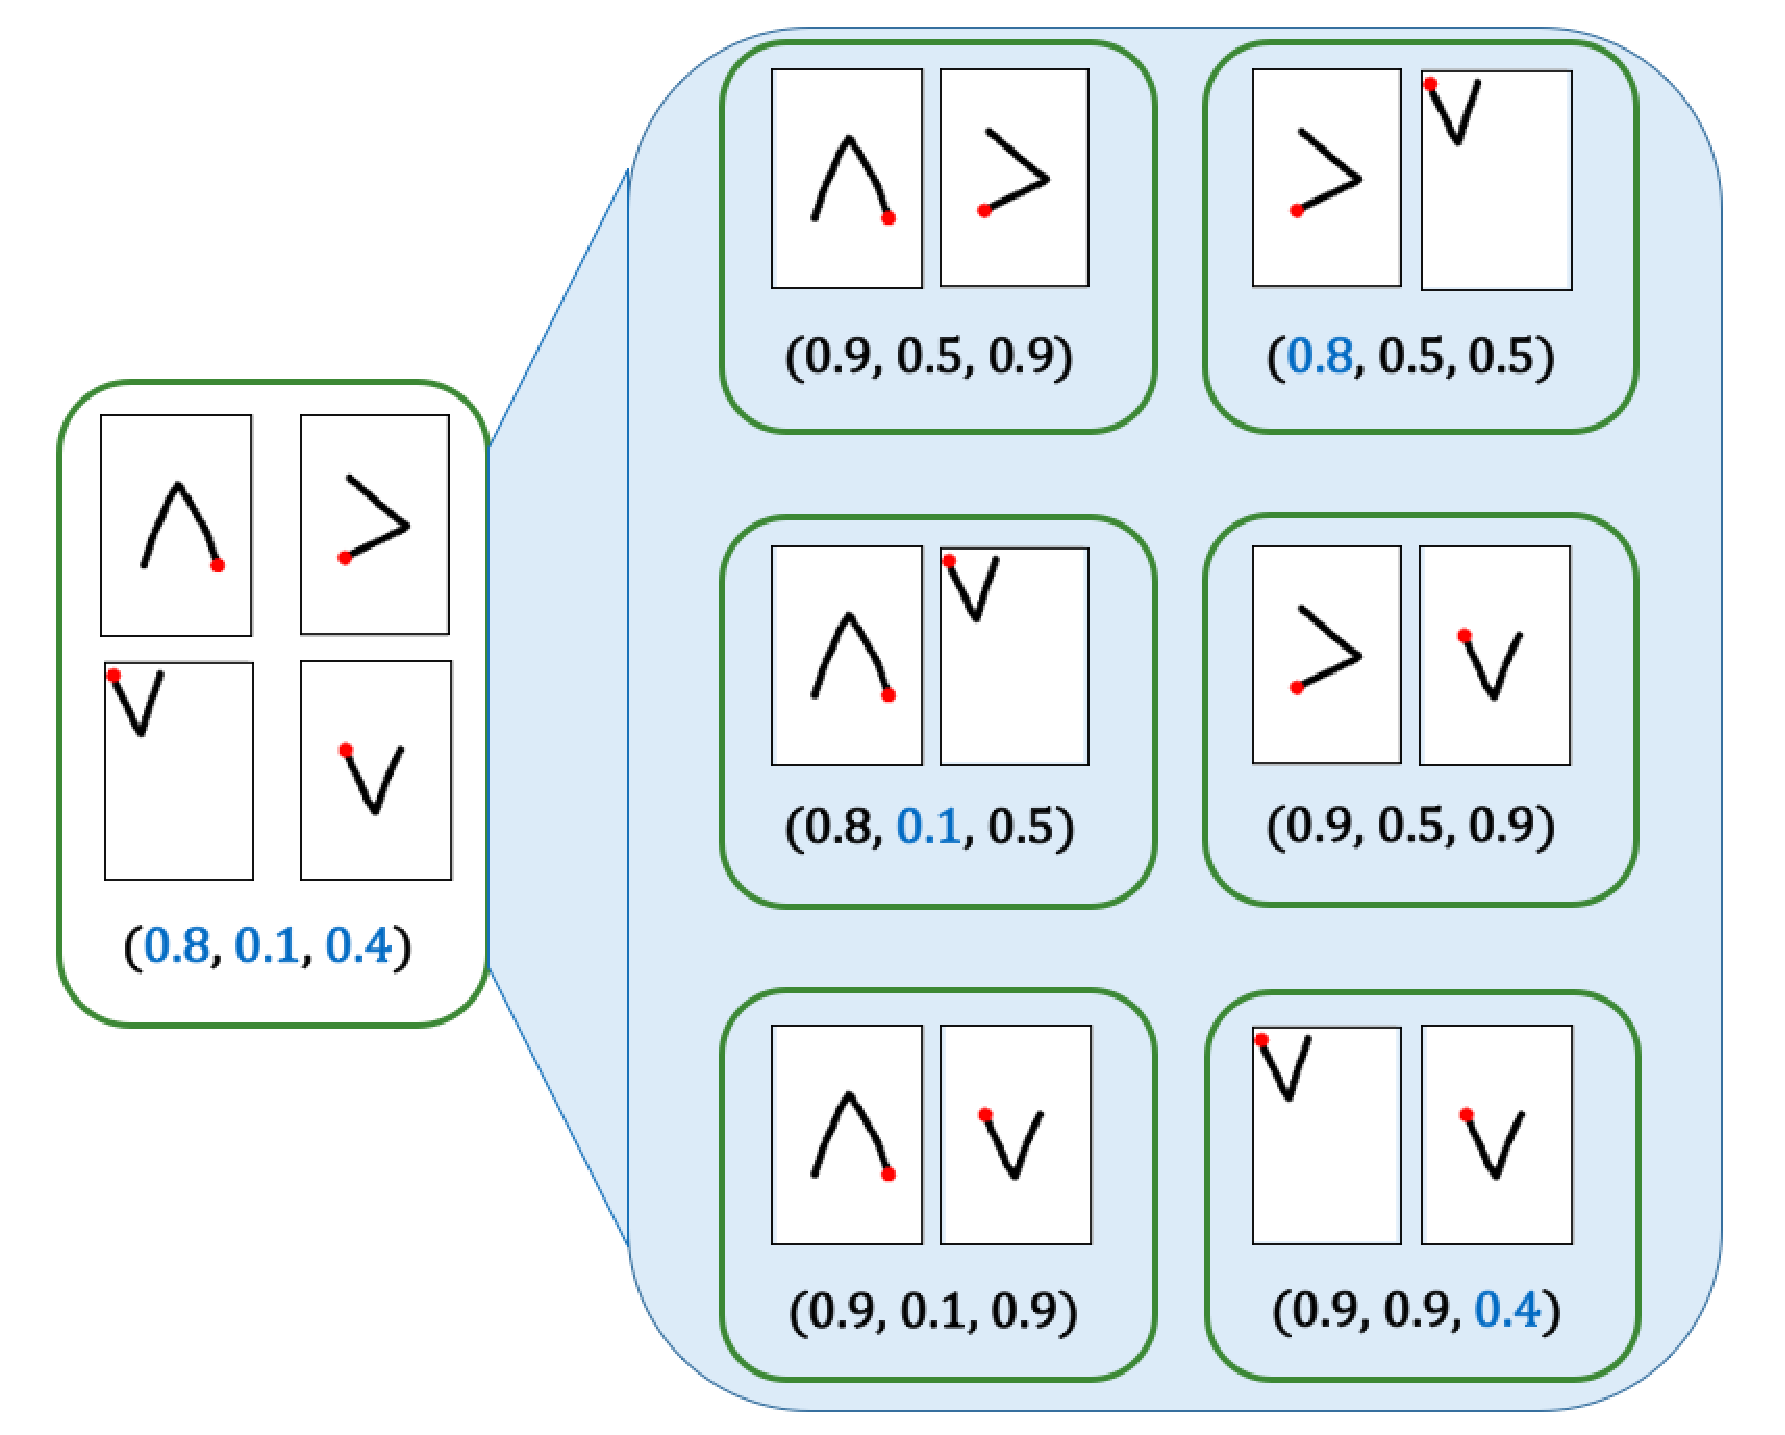
\includegraphics [width=0.8\hsize ]{img/group_similarity.eps}
	\end{center}
	\caption{An Example of how to decide a similarity ($Sts$, $Sto$, $Stp$) of tempaltes in a group gesture, in this case (0.8, 0.1, 0.4) is the similarities.}
	\label{fig:group_similarity}
\end{figure}

以上のようにして得られたジェスチャグループの学習データ間の類似度を用いて,そのジェスチャグループが認識に用いる特徴量を選定する.本実験においては,類似度が0.8を超えた場合において,認識に用いる特徴量として選定した.


\subsection{ジェスチャの認識方法}
入力データの認識方法の手順は2つに分かれている.
\begin{enumerate}
\item \$1アルゴリズムを用いることにより,どのジェスチャグループに属するか判別する.この時,学習データを追加する時と同様,ジェスチャグループ内のすべての学習データに対し類似度を求め,0.8を超えた場合あるいは,0.8を超えるジェスチャが複数存在する場合は,最も類似度が高いジェスチャが存在するジェスチャグループに属すると判別する.
\item ジェスチャグループ内において,どのジェスチャと最も類似しているかを判別する.
\end{enumerate}
2. において,類似度は以下の式によって求められる.
\begin{equation}
S_\textit{final} = S_\textit{cs} \times α_\textit{s} + S_\textit{co} \times α_\textit{o} + S_\textit{cp} \times α_\textit{p}
\end{equation}
\TODO{平均値になるよう修正}

\begin{equation}
α = \left \{
\begin{array}{l}
0 (α>0.8) \\\\
1 (else)
\end{array}
\right.
\end{equation}
ここで\TODO{式の説明}

\subsection{被験者}
被験者は,ユーザ調査において協力してもらった6名である~(男性6名,21〜27歳~(平均23.8歳),全員右利き).

\subsection{実験機器}
実験には,入力端末としてiPhone5を用い,実験における入力領域は1.94'' × 3.18''であり,解像度は640 × 1036である~(図\ref{fig:screenshot}における緑色の部分).

\begin{figure}[!h]
\centering
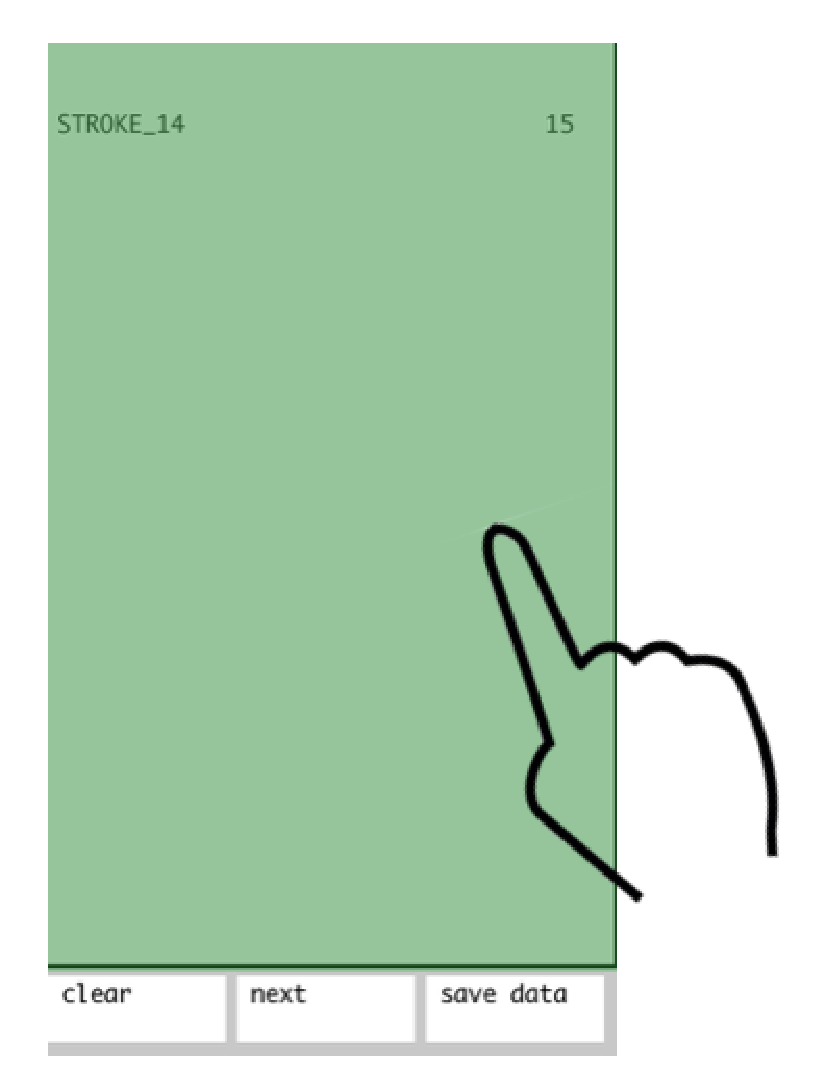
\includegraphics[width=0.4\columnwidth]{img/screenshot.eps}
\caption{The screen shot on the smartphone. The green area is the input area}
\label{fig:screenshot}
\end{figure}


\subsection{実験手順}
\subsubsection{ジェスチャの取得}
我々はまず,被験者に実験の目的を説明した.
その後,ユーザ調査において記入してもらった紙を見ながら,それぞれのジェスチャを入力するよう指示した.
ジェスチャは図\ref{fig:screenshot}における緑色の領域部分にジェスチャを入力するよう指示した.
その際,紙に書かれた,そのジェスチャを入力するときの姿勢に従い入力するよう指示した.
それぞれのジェスチャには,ジェスチャ番号がSTROKE\_1のようにして割り振られており,図\ref{fig:screenshot}に示すように,画面左上に入力すべきジェスチャが表示される.
タスクの1試行は被験者が1つのジェスチャを入力するまでである.被験者はランダムに選択されたそれぞれのジェスチャを1回ずつ入力し,これを1セッションとした.これを10セッション行った.被験者によって入力すべきジェスチャの数は異なるが,いずれの被験者においても20以上のジェスチャを入力する(20〜24個のジェスチャ,平均22個).したがって,被験者は平均して計220試行~(22ジェスチャ $\times$ 10セッション)行った.
ジェスチャが思うように入力できなかった場合には,何度でも書き直し可能とした.

\subsubsection{認識率と認識速度の測定}
それぞれの被験者ごとのジェスチャを``ジェスチャセット''とする.本実験において被験者は6人であるため,ジェスチャセットは6つ存在する.実験はジェスチャセットごとに行うためユーザ依存となる.それぞれのジェスチャは10個ずつあり,学習データをランダムにE個選ぶ.その際のジェスチャグループの決め方と,ジェスチャグループの学習データ間の類似度の計算方法は,〜節に示したとおりである.学習データを追加し終わった後,入力データを残りの10 - E個のジェスチャからランダムに1個選び,認識率と認識速度を測定した~(10分割交差検定).これをそれぞれのジェスチャにつき100回行った.本実験はE = 1〜5とした.また,認識率はジェスチャセットにおける認識率の100回平均を学習データごとに測定し,認識速度は,ジェスチャセット内のすべてのジェスチャを1回ずつ認識し終わるまでに要した時間の100回平均であり,テストに用いるジェスチャをランダムに選ぶ過程は含まれていない.


\subsection{実験結果}
\TODO{あまり認識率が高くない結果を被験者ごとに載せる}

\TODO{認識速度はそこそこ速い結果を載せる}

\subsection{考察}
認識速度についてまず触れる.これは速かった.

認識率が低かった原因を書く.

それぞれの特徴量は,認識に用いられるか用いられないかの二通りに分類され,閾値を設けることにより判別してきたが,同じ名前のジェスチャであったとしても,ランダムに選ばれる学習データによっては,認識に用いられる特徴量が異なる場合があった (閾値によって二通りのいずれかに分類されてしまうため,閾値の設定も難しいといった問題もある).

また,図〜において,向き,位置が認識に用いる特徴量として選ばる可能性が高いが,向きは位置に比べ,学習データ間において,類似度が小さい組み合わせが存在するため~(図\ref{fig:group_similarity}参照),向きの方が位置よりも識別するための特徴量として考慮されるべきではないのかという疑問や,それぞれの特徴量による類似度を,同じ尺度において扱うことができるのかという疑問があった (例えば,大きさの類似度 0.9 と向きの類似度 0.9 は,同じくらい類似していると言えるのかなど).

そこで,これらの問題点に対し,それぞれの特徴量を,認識に用いられるか用いられないかの二通りに分類するのではなく,重み付けを行うことによって解決しようと試みた.例えば,図〜の例を用いる場合,これまでは特徴量を用いるか用いないかであったため,それぞれの特徴量に対する重みの和が1となる場合,~(大きさ,向き,位置)の重みが~(0,0.5,0.5)であったところを,~(0.1,0.6,0.3)といった具合にする.
このように重みを導入することによって,ジェスチャグループ内の学習データ間の類似度から認識に用いる特徴量を,より高い尤度によって決定することを試みた.

%\begin{figure} [h!]
%	\begin{center}
%		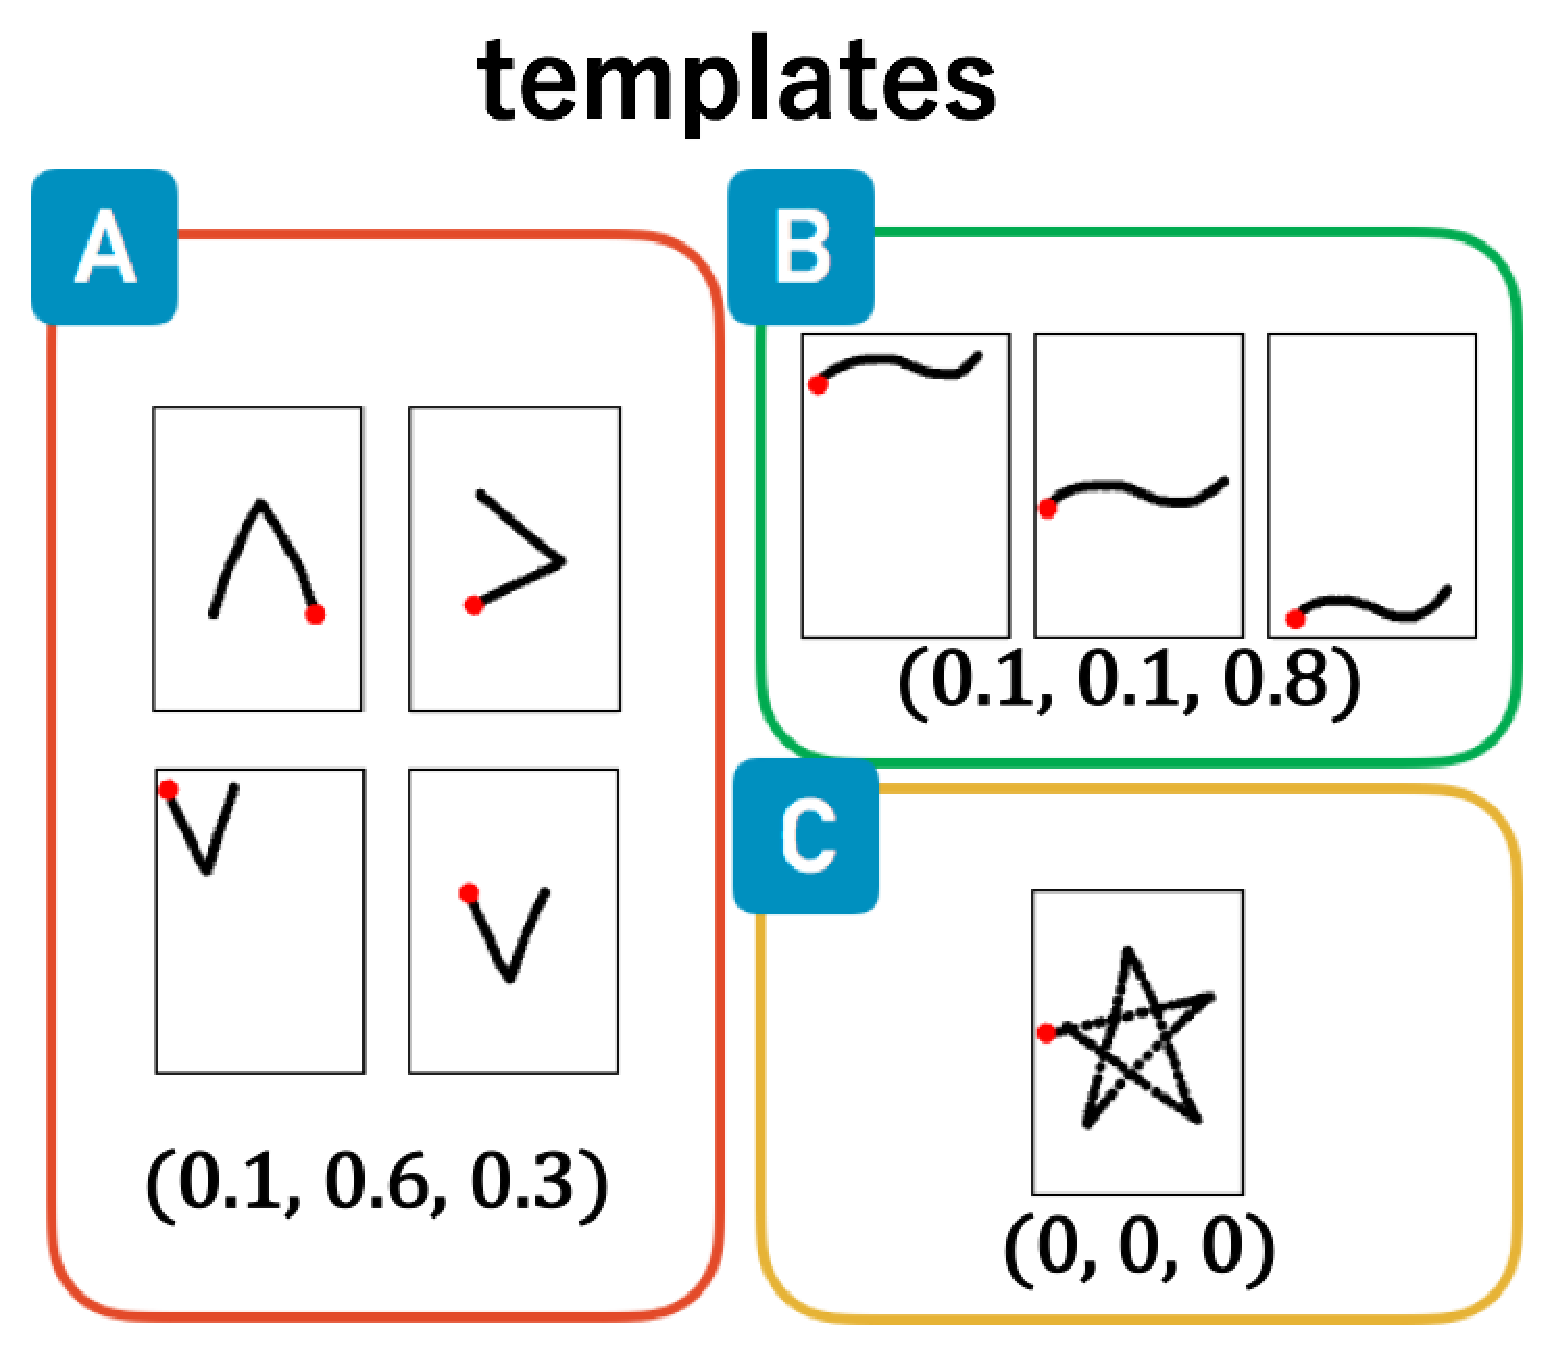
\includegraphics [width=0.7\hsize ]{img/group_weight.eps}
%	\end{center}
%	\caption{Examples of gesture groups and optimal weight values ($Ws$, $Wo$, $Wp$) for each group.}
%	\label{fig:group_weight}
%\end{figure}

\section{最適な重み付けのための実験}
%「同一ジェスチャグループ内において,他の学習データと類似している特徴量は,認識のための特徴量として用いなければ,認識率の低下を防ぐことができる」という仮説
あるジェスチャグループが認識に用いるべき特徴量が,ジェスチャグループの学習データ間の類似度と関係していることは,これまで述べてきた通りである.
そこで我々は,ジェスチャグループの学習データ間の類似度をもとに,認識率を向上させるためのそれぞれの特徴量に対する最適な重み付けの方法を実験的に求めることとした.

\subsection{重み付けの手順}
重み付けの手順を述べる.

学習データは,追加されるたびに,\$1アルゴリズムによりジェスチャグループとして保管される(図\ref{fig:flow}a).この時のジェスチャグループの作成方法は〜において述べた通りである.

一通り学習データを追加し終わった後,テストデータを入力していく.
まず\$1アルゴリズムによりどの形状のジェスチャであるかを判定する.その後「大きさ,向き,位置」のそれぞれの特徴量に対する重みを,それぞれの和が1となるようにそれぞれ0.1ずつ変化させていく.それぞれの重みについて,その形状のジェスチャ内の学習データとのそれぞれの類似度を求め,重みを類似度に乗算することによって,最終的な類似度を求める.
類似度の平均値が0.9以上,N-best Listの1番目と2番目の差が0.2以上の時のそれぞれの特徴量に対する重みを記録する.(図\ref{fig:flow}b)


また,学習データを追加する際,並行して,それぞれの形状ごとに,学習データ間の類似度を求める.類似度は,それぞれの学習データの「大きさ,向き,位置」の特徴量を元に求められ,それぞれ特徴量について最小となった類似度を,その形状のジェスチャの学習データ間の類似度とする.例えば図\ref{fig:flow}a右の場合,「大きさ」は,どの学習データのペアを取ってもさほど変わらないので0.7,「向き」は正反対の学習データのペアが存在するので0.1,「位置」は1つの学習データが他の学習データと比べ比較的異なる位置にあるため,0.5といった具合である.
最小となる類似度を採用する理由は,学習データ内において,1つでも他の学習データと大きく異なる特徴量を持つ学習データが存在すれば,その特徴量を後に認識の際に考慮すべき特徴として扱うべきであると考えたからであり,今後実験によって検討すべき点でもある.

そして,それぞれの形状ごとの学習データ間の類似度と,先ほど記録した重みを比較することによって,どのような特徴を持つ学習データの場合に,どのような重み付けをすることが望ましいかを考察する.

\begin{equation}
S{\tiny f} = S{\scriptsize cs} \times W{\scriptsize s} + S{\scriptsize co} \times W{\scriptsize o} + S{\scriptsize cp} \times W{\scriptsize p}
\end{equation}

\begin{figure} [h!]
	\begin{center}
		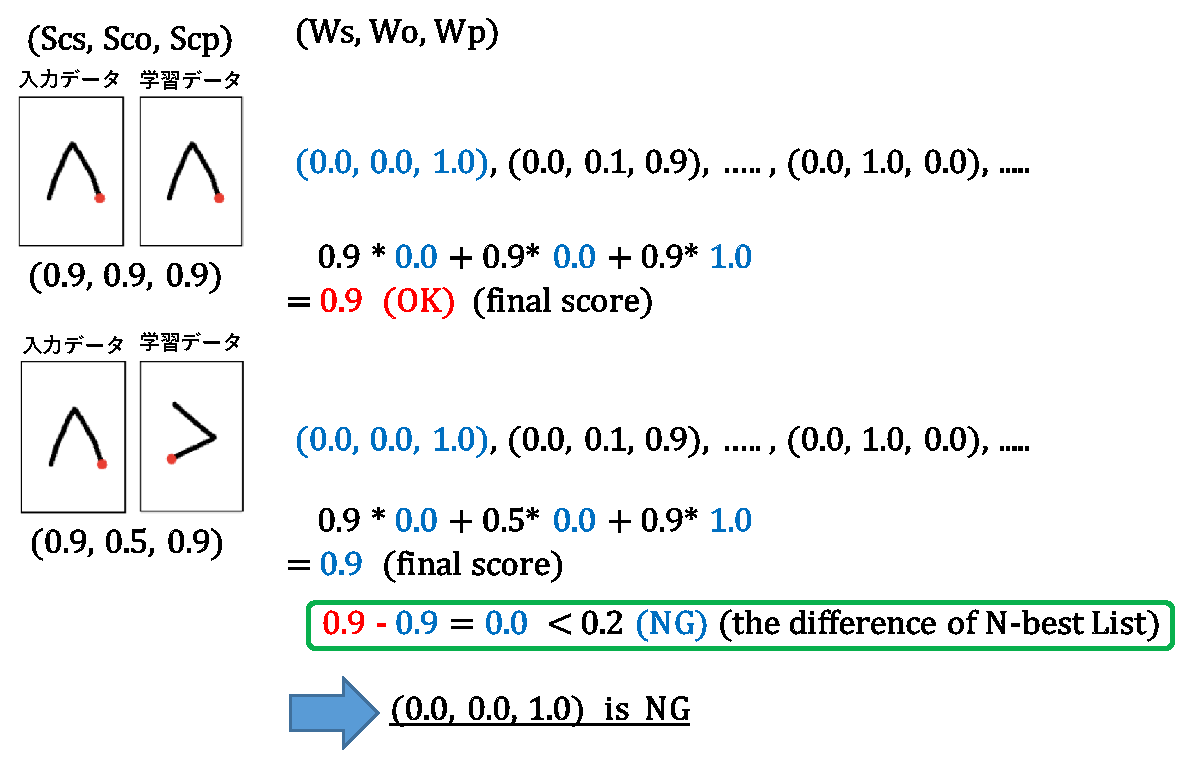
\includegraphics [width=0.8\hsize ]{img/weight_method1.eps}
	\end{center}
	\caption{The procedure to decide the optimal weight values }
	\label{fig:weight_method1}
\end{figure}

\begin{figure} [h!]
	\begin{center}
		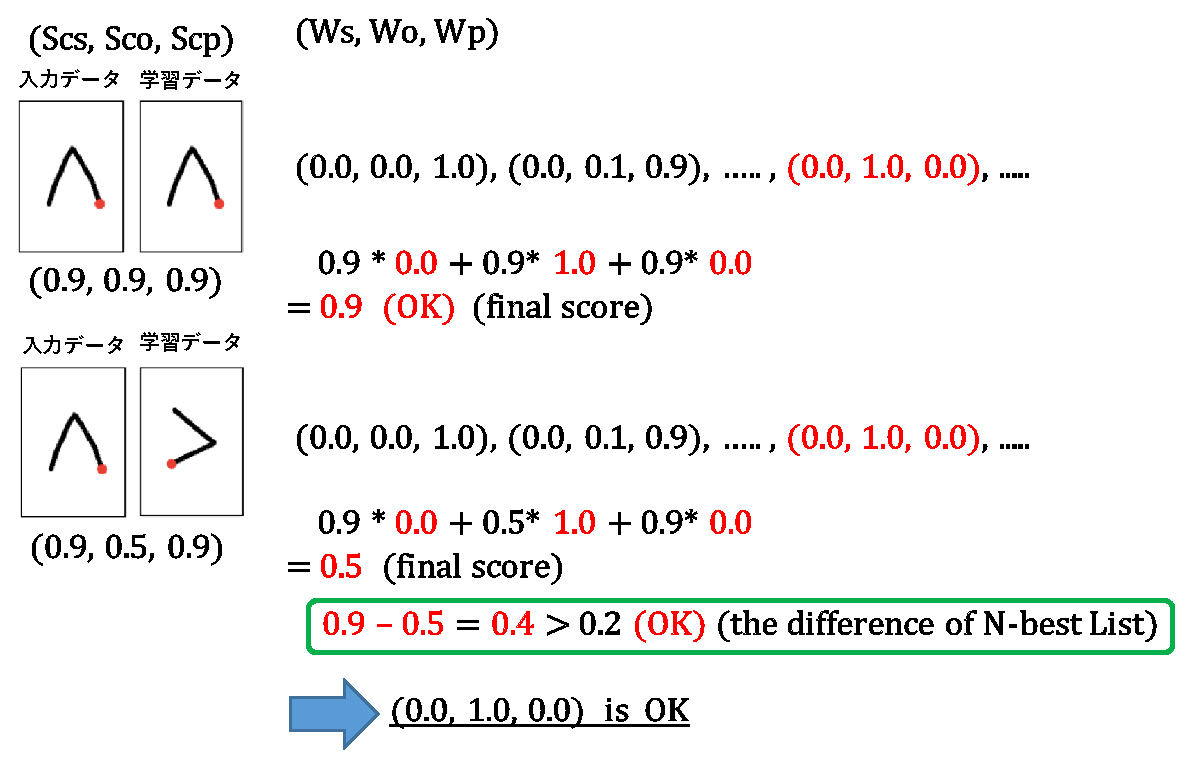
\includegraphics [width=0.8\hsize ]{img/weight_method2.eps}
	\end{center}
	\caption{The procedure to decide non optimal weight values}
	\label{fig:weight_method2}
\end{figure}

\subsection{実験結果}
\begin{figure*} [t]
 \begin{center}
  \includegraphics [width=1.0\columnwidth]{img/weight_graph.eps}
  \caption{The result of the experiment to find the optimal weight values, and blue lines indicates power approximation curves.}
  \label{fig:weight_graph}
 \end{center}
\end{figure*}

\section{ジェスチャの認識}


